%        File: paper.tex
%     Created: Fri Jun 23 06:00 PM 2017 J
% Last Change: Fri Jun 23 06:00 PM 2017 J
%
\input{../EMSOFT2016/dummy/dummy.tex}
\documentclass[submit]{ipsj_v2/UTF8/ipsj}

\usepackage{latexsym}
\usepackage[dvipdfmx]{graphicx}
\usepackage{amssymb}
\usepackage{enumerate,cite,url}
\usepackage{listings,jlisting}
\lstset{%
    language={c},%
    basicstyle={\small},%
    identifierstyle={\small},%
    commentstyle={\scriptsize\itshape},%
    keywordstyle={\small},%\bfseries},%
    ndkeywordstyle={\small},%
    stringstyle={\small\it},
    frame={tb},
    breaklines=true,
    columns=[l]{fullflexible},%
    numbers=left,%
    xrightmargin=0zw,%
    xleftmargin=3zw,%
    numberstyle={\scriptsize},%
    stepnumber=1,
    numbersep=1zw,%
    lineskip=-0.5ex%
}

\begin{document}

\title{組込みシステムに適した\\動的メモリアロケータのコンポーネント化}

\etitle{Componentized Dynamic Memory Allocator for Embedded Systems}

\affiliate{OU}{大阪大学基礎工学研究科\\
Graduate School of Engineering Science, Osaka University}

\affiliate{OKUMA}{オークマ株式会社\\
OKUMA Corporation}

\author{山本 拓朗}{Takuro Yamamoto}{OU}%[joho.taro@ipsj.or.jp]
\author{大山 博司}{Hiroshi Oyama}{OKUMA}%
\author{安積 卓也}{Takuya Azumi}{OU}%[gakkai.jiro@ipsj.or.jp]

\maketitle

\section{はじめに}
近年,組込みシステムは多くの機器に組み込まれており,このIoT社会を支える重要な役割を担っている.
多くの組込みシステムは,厳しいリソース制約を持っており,効率的なメモリ確保が要求される.
さらに,リアルタイム性を要求される組込みシステムでは,メモリ確保の実行時間も重要となる.

このような要求を満たす,組込みシステムに適した動的メモリアロケータとして,TLSF (Two-Level Segregate Fit) アロケータが提案されている.
TLSFアロケータは,メモリブロックを2段階で分類することでメモリ利用効率を向上させており,常にオーダー1で実行するため最悪実行時間が存在しない.
TLSFアロケータは,メモリ利用効率が良く,リアルタイムシステムに向いているため,多くのリアルタイムOSで利用されている.

しかし,現状では,複数のスレッドが並行動作すると,メモリの衝突が起きる場合がある.
本研究では,組込み向けコンポーネントシステムであるTECS (TOPPERS Embedded Component System) を用いてTLSFアロケータをコンポーネント化する.
コンポーネント化されたTLSFアロケータでは,各コンポーネントで独自のヒープ領域を保持するため,スレッドセーフなアロケータを実現できる.
さらに,コンポーネントとして特性を利用できるため,メモリサイズの変更等が柔軟になる.
本論文では,提案するTLSFメモリアロケータコンポーネントのユースケースとして,利用例を述べる.

% 本論文における貢献は以下の通りである.
% \begin{enumerate}
%
% \end{enumerate}

本論文の構成は次の通りである.
まず\ref{sec:ComponentBasedDevelopment}章で,コンポーネントベース開発と提案するアロケータのベースとして用いるTECSについて述べる.
\ref{sec:Design and Implementation}章では,TLSFアロケータのコンポーネント設計と実装について述べる.
\ref{sec:Use Case}章では,ユースケースとして,利用例を述べる.
\ref{sec:Related Work}章では,関連研究を述べ,最後に\ref{sec:Conclusion}章で本論文をまとめる.

\section{コンポーネントベース開発}
\label{sec:ComponentBasedDevelopment}

ソフトウェア開発の生産性を向上させる手法のひとつにコンポーネントベース開発がある.
コンポーネントベース開発は,ソフトウェアの部品(コンポーネント)を組み合わせて開発を行う手法である.
ソフトウェアの再利用性が改善する上に,コンポーネント図によりシステム全体の構造を可視化するため,ソフトウェア開発の生産性を向上できる.
さらに,システムの拡張や仕様変更にも柔軟に対応することができる.

\subsection{TECS}
TECS (TOPPERS Embedded Component System)は,TOPPERSプロジェクトで開発されている組込みシステム向けのコンポーネント技術である.
TECSでは,コンポーネントの生成と結合はすべて静的に行われ,最適化されるため,コンポーネント化における実行時間や消費メモリのオーバヘッドを抑えることができる.
% 他の特徴として,C言語での実装,ソースレベルでの移植性,コンポーネントの粒度が小さいことなどがある.

\subsubsection{コンポーネントモデル}
図\ref{fig:component}にTECSコンポーネント図の例を示す.
TECSでは,インスタンス化されたコンポーネントはセル({\it cell})と呼ばれ,受け口({\it entry}),呼び口({\it call}),属性,変数を持つ.
受け口は自身の機能を提供するインタフェースで,呼び口は他のセルの機能を利用するためのインタフェースである.
セルは複数の受け口や呼び口を持つことができる.
セルの提供する関数は,C言語で実装される.

受け口と呼び口の型は,セルの機能を使うためのインタフェースであるシグニチャによって定義される.
セルの呼び口は,同じシグニチャを持つ他のセルの受け口と結合できる.
セルの型は,セルタイプと呼ばれ,受け口,呼び口,属性,変数の組を定義している.

\begin{figure}[t]
    \centering
    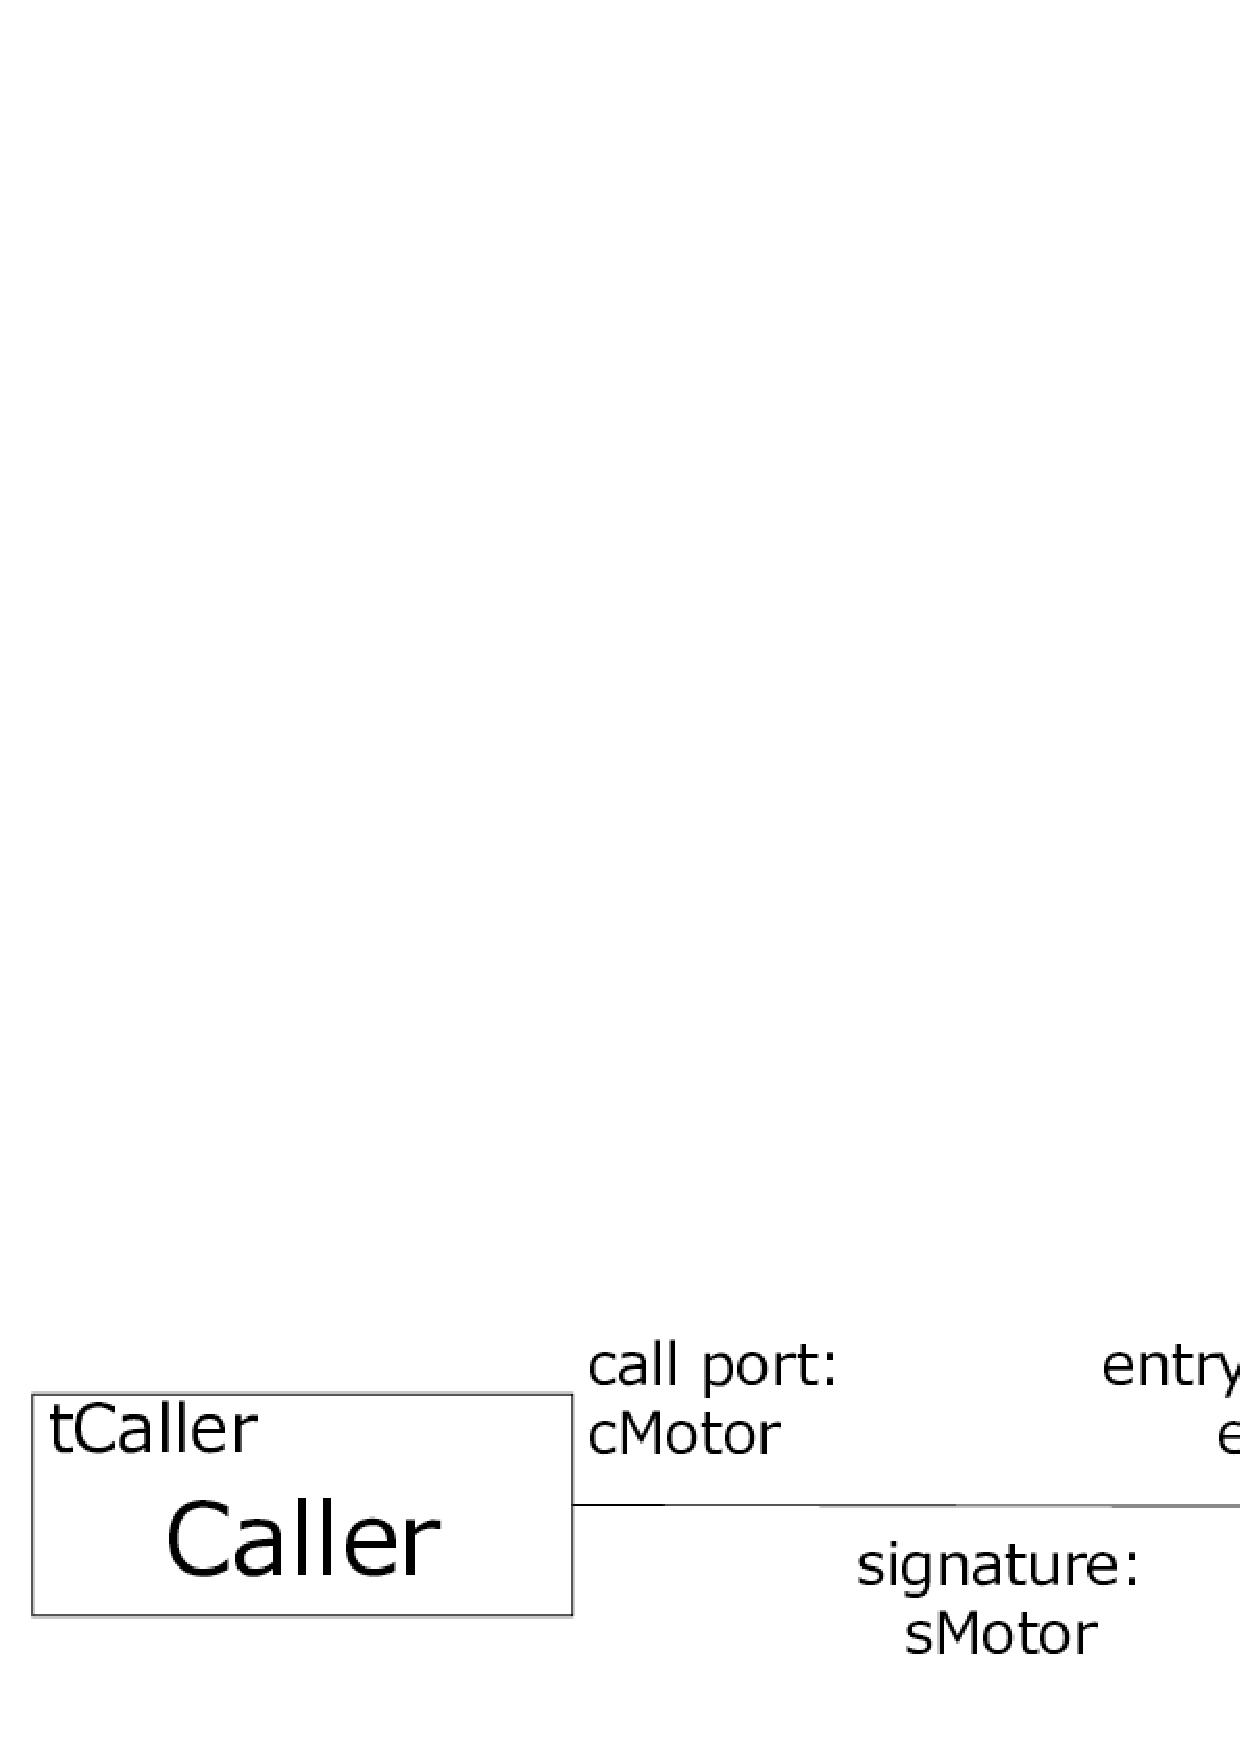
\includegraphics[width=8cm,clip]{figure/component_diagram.pdf}
    \caption{TECSコンポーネント図の例}
    \label{fig:component}
\end{figure}

\subsubsection{コンポーネント記述}
TECSのコンポーネント記述は,シグニチャ記述,セルタイプ記述,組上げ記述に分類され,cdlファイルに記述する.
図\ref{fig:component}のコンポーネント記述について次に述べる.

\begin{description}
    \item[{\bf シグニチャ記述}]\mbox{}\\
        シグニチャ記述は,セルのインタフェースを定義する.
        図\ref{signature}に示す通り,{\it signature}キーワードに続けて,シグニチャ名(sMotor)を記述する.
        %図\ref{signature}のようにシグニチャsMotorを定義できる.
        TECSでは,インタフェースの定義を明確にするために,入力と出力にはそれぞれ,[in]と[out]という指定子が付けられる.
        
\begin{figure}[t]
\centering
\begin{lstlisting}
signature sMotor {
    int32_t getCounts( void );
    ER resetCounts( void );
    ER setPower( [in]int power );
    ER stop( [in] bool_t brake );
    ER rotate( [in] int degrees, [in] uint32_t speed_abs,
              [in] bool_t blocking );
    void initializePort( [in]int32_t type );
};
\end{lstlisting}
\caption{シグニチャ記述}
\label{signature}
\end{figure}

    \item[{\bf セルタイプ記述}]\mbox{}\\
        セルタイプ記述は,受け口,呼び口,属性,変数を用いてセルタイプを定義する.
        {\it celltype}キーワードに続けて,セルタイプ名(tCaller)を記述する.
        図\ref{celltype}に示す通り,受け口は,{\it entry}キーワードに続けて,シグニチャ名,受け口名を記述する.
        同様にして,呼び口も定義できる.
        属性と変数は,それぞれ{\it attr},{\it var}キーワードを用いて列挙する.

\begin{figure}[t]
\centering
\begin{lstlisting}
celltype tCaller {
    call sMotor cMotor;
};
celltype tMotor {
    entry sMotor eMotor;
    attr {
        int32_t attr = 100;
    };
    var {
        int32_t var;
    };
};
\end{lstlisting}
\caption{セルタイプ記述}  
\label{celltype}
\end{figure}

    \item[{\bf 組上げ記述}]\mbox{}\\
        組上げ記述は,セルをインスタンス化し,セルを結合する.
        {\it cell}キーワードに続けて,セルタイプ名,セル名を記述する.
        呼び口名,``=",結合先の受け口名の順に記述し,セルを結合する.
        図\ref{build}では,セルCallerの呼び口cMotorと,セルMotorの受け口eMotorが結合されている.
        
\begin{figure}[t]
\centering
\begin{lstlisting}
cell tMotor Motor {
};
cell tCaller Caller {
    cMotor = Motor.eMotor;
};
\end{lstlisting}
\caption{組上げ記述}
\label{build}
\end{figure}

\end{description}

\section{設計と実装}
\label{sec:DesignImplementation}

本章では,TLSFアロケータのコンポーネント設計について述べる.
% 図\ref{fig:TLSFComponent}に,コンポーネント化されたTLSFアロケータのコンポーネント図を示す.


\subsection{TLSF}
\label{sec:TLSF}
TLSF (Two-Level Segregate Fit)アロケータは,M. Masmanoらによって提案されたリアルタイムシステムに適した動的メモリアロケータである.

\begin{figure}[t]
\centering
\begin{lstlisting}
[deviate]
signature sMalloc {
    int    initializeMemoryPool(void);
    void   *calloc( [in]size_t nelem, [in]size_t elem_size );
    void   *malloc( [in]size_t size );
    void   *realloc( [in]const void *ptr, [in]size_t new_size );
    void   free( [in]const void *ptr );
};
\end{lstlisting}
\caption{メモリ管理用のシグニチャ記述}  
\label{src:TLSFSignature}
\end{figure}

\begin{figure}[t]
\centering
\begin{lstlisting}
celltype tTLSFMalloc {
    [inline]
        entry  sMalloc  eMalloc;
    attr {
        /* memory pool size in bytes */
        size_t  memoryPoolSize;
    };
    var {
        [size_is( memoryPoolSize / 8 )]
            uint64_t   *pool;
    };
};
\end{lstlisting}
\caption{TLSFアロケータのセルタイプ記述}  
\label{src:TLSFCelltype}
\end{figure}

\section{ユースケース}
\label{sec:UseCase}

本章では,提案するコンポーネント化されたTLSFメモリアロケータのユースケースとして,利用されるプラットフォームとその効果について述べる.

\subsection{mruby on TECS}
\label{sec:mrubyonTECS}

mruby on TECS は,mruby (軽量Ruby)を用いたコンポーネントベース開発が可能な組込みソフトウェア開発フレームワークである.
スクリプト言語を用いることで,組込みソフトウェア開発の生産性向上を目指している.
一般に,スクリプト言語は実行速度が遅いため,組込みソフトウェアに向いていないが,mruby on TECSでは,mruby-TECSブリッジの機能によって,mruby プログラムからC 言語の関数を呼び出すことができるため,C言語と変わらない速度でプログラムを実行することができる.
mrubyプログラムは,mrubyコンパイラによってバイトコードに変換され,RiteVMと呼ばれるVM上で実行される.
本フレームワークでは,RiteVMやRTOS (Real-Time OS)の機能もすべてTECSによってコンポーネント化されている.

% 本研究では,RTOS として,TOPPERS/HRP2 [6] を使用した.
% TOPPERS/HRP2 は,$\mu$ITRONをベースにしたメモリ保護機能を持つRTOSである.
% しかし,TECSはTOPPERS/HRP2 だけでなく,OSEKやTOPPERS/ASPといったRTOS にも対応しているため,mruby on TECS はRTOS に依存しない.

\subsubsection{マルチVM対応}

本フレームワークでは,VMが行うメモリ管理にTLSFメモリアロケータを採用している.
しかし,既存のTLSFメモリアロケータではスレッドセーフではないため,複数のスレッドからメモリの確保や解放を行うと,メモリ衝突が起きてしまう.
VMは高い頻度でメモリの確保と解放を繰り返すため,マルチVMとして複数のVMを起動すると,すぐに衝突を起こしてしまう.

図\ref{fig:TLSF-mruby}のように,VMにTLSFメモリアロケータコンポーネントを結合し,各VMで独自のヒープ領域を持つように設計する.
各VMがそれぞれメモリプールを保持しているため,複数のVMがメモリ衝突を起こすことなく,実行できる.
さらに,RiteVMはインクリメンタルGC (Garbage Collection)を行うが,独自のメモリプールを保持しているため,GCを始めたVMがGCの実行によって,他のVMの実行を妨げることもない.
    
\subsection{TINET+TECS}
\label{sec:TINET+TECS}

TINET+TECSは,組込み向けのTCP/IPプロトコルスタックであるTINET (Tomakomai InterNETworking)をTECSによってコンポーネント化したTCP/IPプロトコルスタックである.

\section{関連研究}
\label{sec:RelatedWork}

\section{おわりに}
\label{sec:Conclusion}

%%%%%%%%%%%% Reference %%%%%%%%%%%%%%%%%%%%%%%%%%%%%%%%%%%%%%%%%%%%%%
\bibliographystyle{ipsj_v2/UTF8/ipsjunsrt-e}
\bibliography{ref}

% \begin{biography}
% \profile{m,E}{情報 太郎}{1970年生.1992年情報処理大学理学部情報科学科卒業.
% 1994年同大学大学院修士課程修了.同年情報処理学会入社.オンライン出版の研究
% に従事.電子情報通信学会,IEEE,ACM 各会員.}
% %
% \profile{n}{処理 花子}{1960年生.1982年情報処理大学理学部情報科学科卒業.
% 1984年同大学大学院修士課程修了.1987年同博士課程修了.理学博士.1987年情報処
% 理大学助手.1992年架空大学助教授.1997年同大教授.オンライン出版の研究
% に従事.2010年情報処理記念賞受賞.電子情報通信学会,IEEE,IEEE-CS,ACM
% 各会員.}
% %
% \profile{h,L}{学会 次郎}{1950年生.1974年架空大学大学院修士課程修了.
% 1987年同博士課程修了.工学博士.1977年架空大学助手.1992年情報処理大学助
% 教授.1987年同大教授.2000年から情報処理学会顧問.オンライン出版の研究
% に従事.2010年情報処理記念賞受賞.情報処理学会理事.電子情報通信学会,
% IEEE,IEEE-CS,ACM 各会員.}
% \end{biography}

\end{document}
